\section{Introduction}

This document is to summarise the experiments attempted to bias the seeding procedure of CC2538\cite{CC2538_Manual} manufactured by TI.

The greatest difficulty in this project is that TI did not disclose details of how the seeding is done. The only descriptions in CC2538 User's Guide are:
\begin{quote}
...For the CC2538, when a random value is required, writing the SOC\_ADC\_RNDL register with random bits from the IF\_ADC in the RF receive path seeds the LFSR. To use this seeding method, first power on the radio. The radio must be placed in the infinite RX state to avoid possible sync detect in the RX state.The random bits from the IF\_ADC are read from the LSB position of the RF register RFCORE\_XREG\_RFRND. These bits should be concatenated over time to form the bytes needed for the RNG seed... This cannot be done while the radio is in use for normal tasks... (Section 16.2.2, CC2538 User's Guide)

...The RF Core can generate random bits. The chip should be in RX when generation of random bits is required. One must also make sure that the chip has been in RX long enough for the transients to have died out. A convenient way to do this is to wait for the RSSI-valid signal to go high. Single random bits from either the I or Q channel can be read from the RFRND register... (Section 23.12, CC2538 User's Guide)
\end{quote}

\Cref{CC2538_RFRND} shows the description of the crucial RFRND register in the manual of CC2538.

\begin{figure}
\center
\caption{Description of RFRND from CC2538 User's Guide}
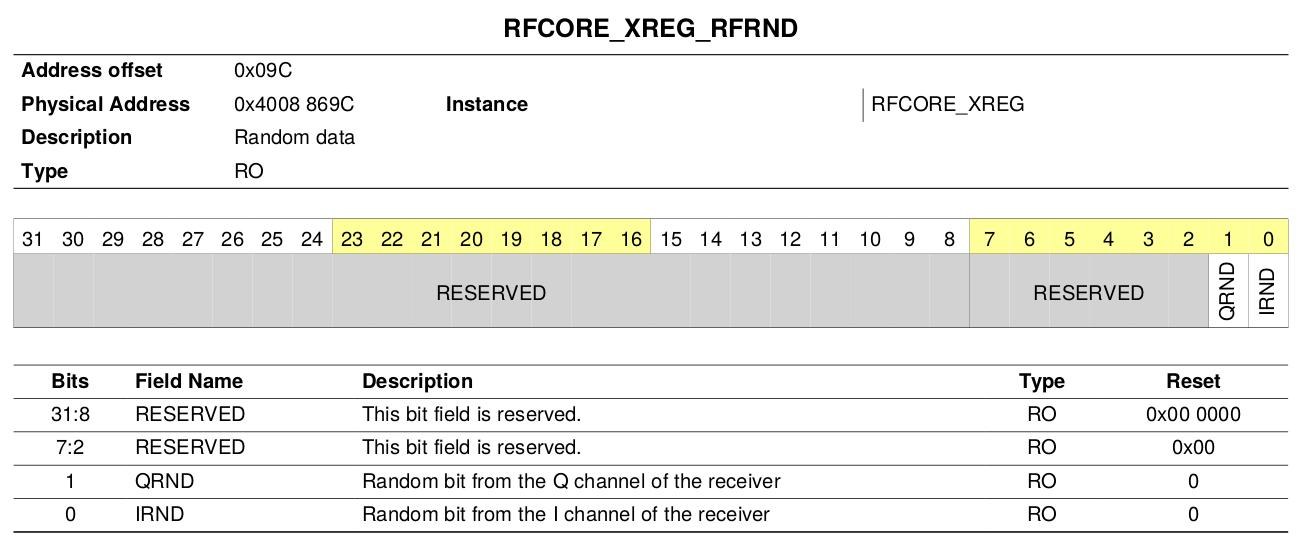
\includegraphics[width=\linewidth]{./figures/CC2538_RFRND.png}
\label{CC2538_RFRND}
\end{figure}

In conclusion, the manual tells us:
\begin{enumerate}
\item The random bits are derived from the IQ channels of IF\_ADC in the receive path, one bit at once, accessed through RFRND register.
\item The random bits are not available until the transients of IF\_ADC has died out.
\end{enumerate}

From a security perspective, seeding with the RF module leads to the suspect that is it possible to create bias in the seed by manipulating IF\_ADC through radio signals? There are several critical questions those are not documented but crucial in answering this suspect:
\begin{enumerate}
\item How does IF\_ADC converts to a random bit?
\item Why infinite RX state is required?
\item Does RSSI play a role in the procedure? If yes, how?
\item What are the electronic characteristics? Including what is the IF, sample rate, etc.
\end{enumerate}

In this report, we mainly took two approaches to carry on the research:
\begin{enumerate}
\item Searching for related contents in the documents of product in the same series as they may shared the same design.
\item Black box experiments.
\end{enumerate}

CAUTION: Since the statements in this report are based on empirical document studies and black box experiments; thus they might not be accurate. As of writing this report, we have not yet successfully biased the seed.

\section{Related Documents Study}

CC2538, launched in May 2013, is not the first product that adopts the design of using RF to seed its PRNG, which is a 16-bit CRC16 LSFR register. The same seeding and PRNG design can trace back to one of its predecessor CC2430\cite{CC2430_Manual}, launched in 2007,  where a RNG failure has been reported by  \cite{CC2430Fail}.

In CC2430 User's Guide, we found the following instructions:
\begin{quote}
...When a true random value is required, the LFSR should be seeded by writing RNDL with random values from the IF\_ADC in the RF receive path. To use this seeding method, the radio must first be powered on by enabling voltage regulator as described in section 15.1. The radio should be placed in infinite TX\footnote{This is actually a typo. The RF needs to be in infinite RX state to use this seeding method.} state, to avoid possible sync detect in RX state. The random values from the IF\_ADC are read from the RF registers ADCTSTH and ADCTSTL (see page 196). The values read are used as the seed values to be written to the RNDL register as described above. Note that this can not be done while radio is in use for normal tasks... (Section 13.11.2.2, CC2430 User's Guide)
\end{quote}

We can see that CC2538 User's Guide basically inherited the same sentences, except that the seed is instead read from different registers, ADCTSTH and ADCTSTL. \Cref{CC2430_ADCTST} shows the detailed description of these registers in its manual.

\begin{figure}
\center
\caption{Description of ADCTSTH and ADCTSTL from CC2430 User's Guide}
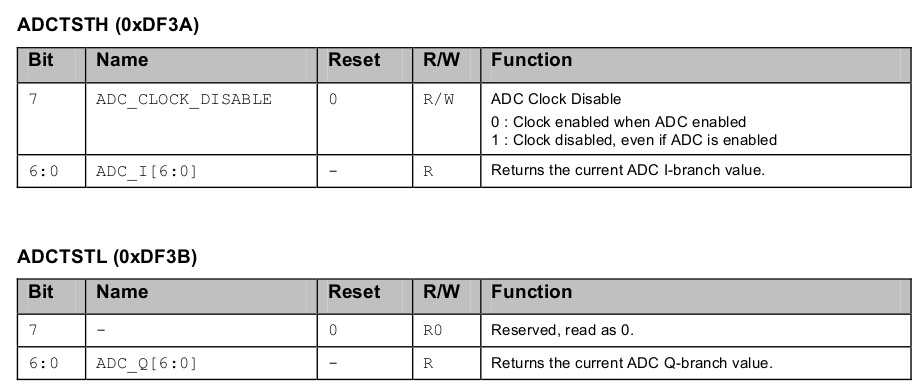
\includegraphics[width=\linewidth]{./figures/CC2430_ADCTST.png}
\label{CC2430_ADCTST}
\end{figure}

Comparing to CC2538, CC2430 User's Guide explains that the ADCs have resolution of 7-bits and one of the IQ channel readings is suggested to be directly used as the random seed. One thing might be worthy pointing out is that the entropy test in \cite{CC2430Fail} may have incorrectly interpreted these 7-bits readings as a byte, even though it does not change the fact that such seed is strongly biased.

CC2430 also disclosed more details about its RF. \Cref{CC2430_RF} provides an overview of its RF design.  We can see that the random seed from IF\_ADC is indeed the output of mixer after band pass filter and AGC, where LO is implemented by the Frequency Synthesiser.

\begin{figure}
\center
\caption{Radio and Demodulator of CC2430 from CC2430 User's Guide}
\begin{subfigure}{\linewidth}
%	\subcaption{Block Diagram of Radio Module from CC2430 User's Guide}
	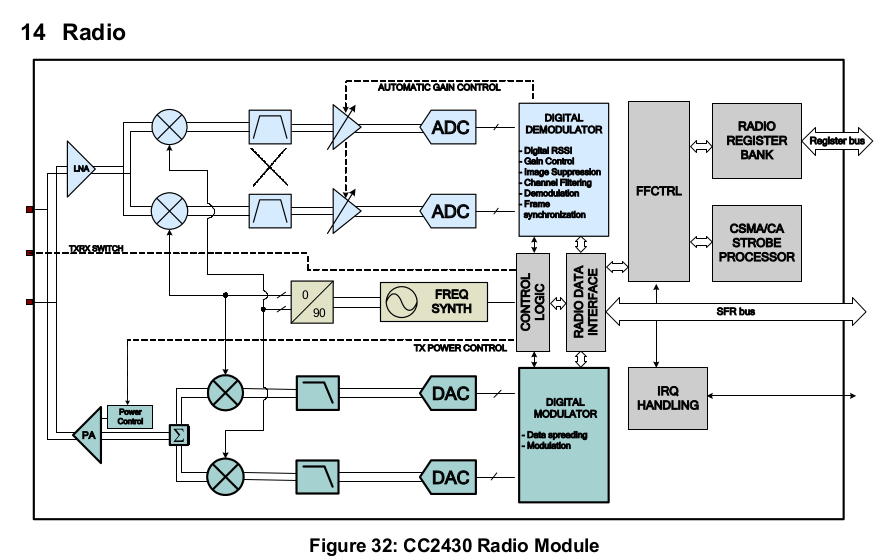
\includegraphics[width=\linewidth]{./figures/CC2430_Radio.png}
\end{subfigure}

\begin{subfigure}{\linewidth}
%	\subcaption{Block Diagram of Demodulator from CC2430 User's Guide}
	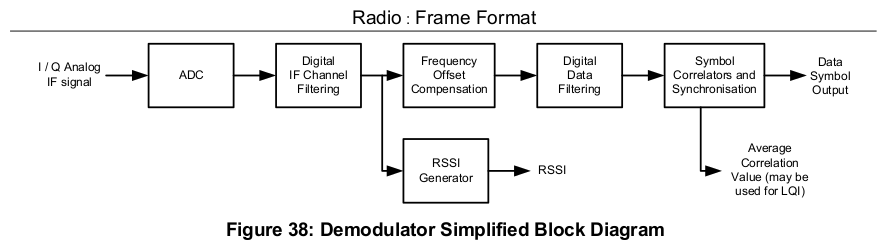
\includegraphics[width=\linewidth]{./figures/CC2430_Demodulator.png}
\end{subfigure}
\label{CC2430_RF}
\end{figure}

The CC253X and CC2540/41 series\cite{CC253X_Manual} is another sibling of CC2538 launched in April 2009. This series also inherited the similar RNG design from CC2430, using a CRC16 register as PRNG seeded by IF\_ADC.

\begin{quote}
...For the CC253x, when a random value is required, the LFSR should be seeded by writing RNDL with random bits from the IF\_ADC in the RF receive path. To use this seeding method, the radio must first be powered on. The radio should be placed in the infinite RX state to avoid possible sync detect in the RX state. The random bits from the IF\_ADC are read from the least-significant bit position of the RF register RFRND. These bits should be concatenated over time to form the bytes needed for the random-number-
generator seed... (Section 14.2.2, CC253X, CC2540/41 User's Guide)
\end{quote}

\Cref{CC253X_RFRND} shows the RFRND register for CC253X.

\begin{figure}
\center
\caption{Description of RFRND from CC253X, CC2540/41 User's Guide}
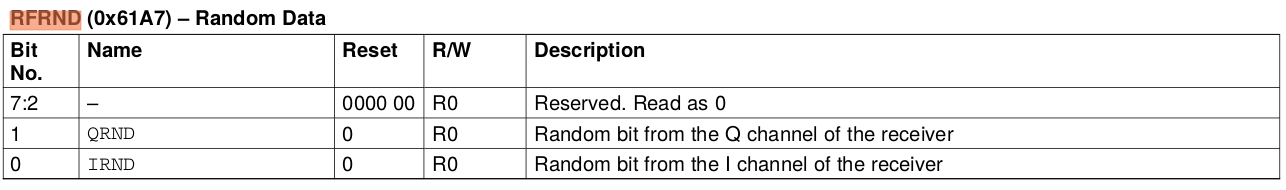
\includegraphics[width=\linewidth]{./figures/CC253X_RFRND.png}
\label{CC253X_RFRND}
\end{figure}

Further inspecting the documents, we realised that CC253X and CC2538 reported exactly identical seeding result in their manuals, as shown in \Cref{CC2538_CC253X_SeedComparison}. This suggests that CC2538 and CC253X are likely used the same RF module.

\begin{figure}
\center
\caption{Seeding Result for CC253X and CC2538}
\begin{subfigure}{0.8\linewidth}
	\subcaption{Seeding Result from CC253X,CC2540/41 User's Guide}
	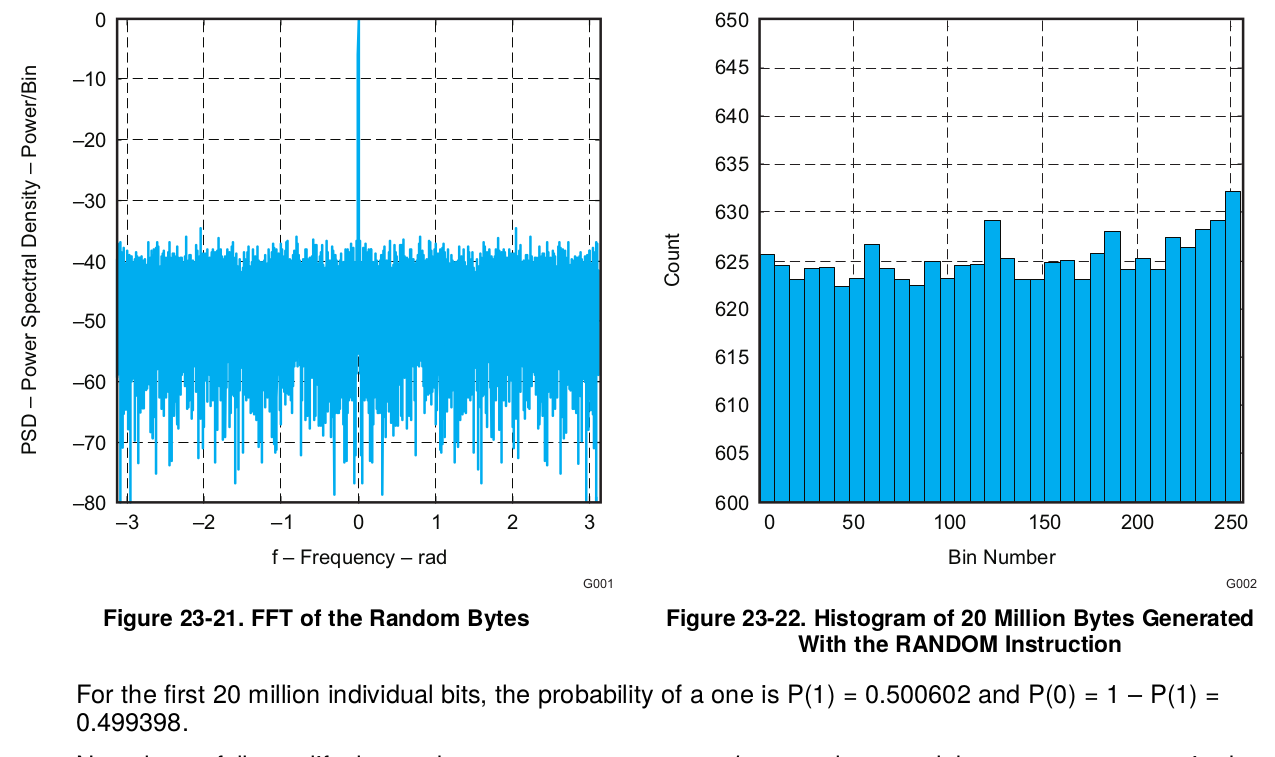
\includegraphics[width=\linewidth]{./figures/CC253X_Seed.png}
\end{subfigure}

\begin{subfigure}{0.8\linewidth}
	\center
	\subcaption{Seeding Result from CC2538 User's Guide}
	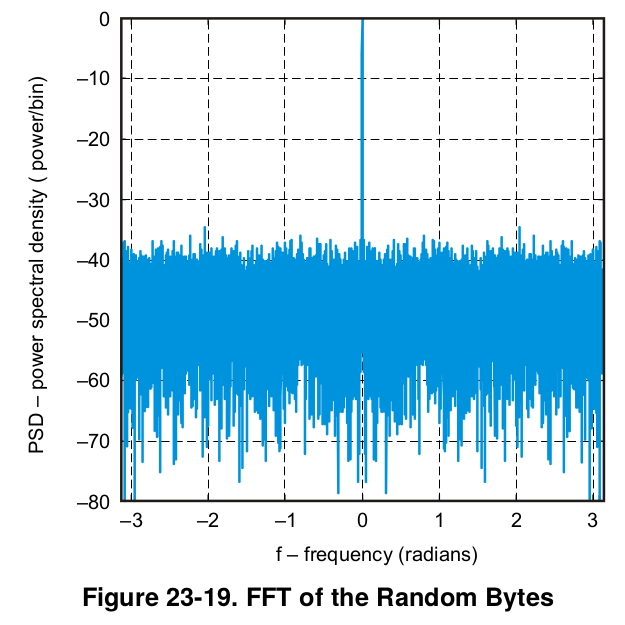
\includegraphics[width=0.55\linewidth]{./figures/CC2538_Seed1.png}
	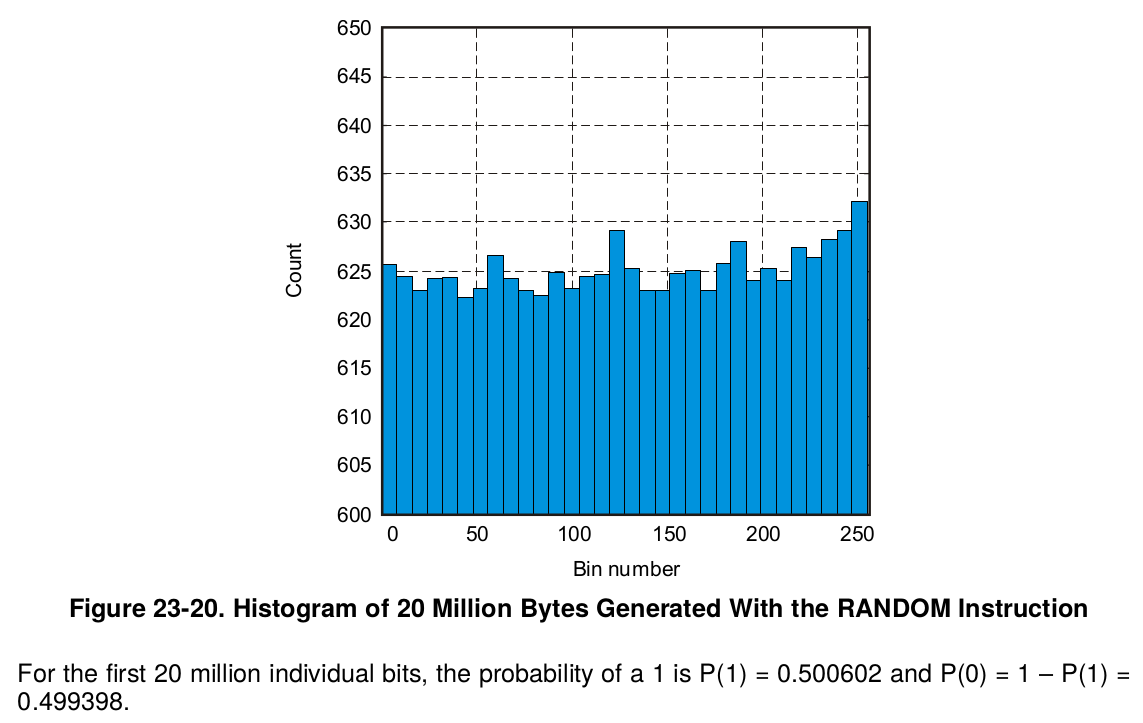
\includegraphics[width=\linewidth]{./figures/CC2538_Seed2.png}
\end{subfigure}
\label{CC2538_CC253X_SeedComparison}
\end{figure}

But the problem remains that neither CC253X nor CC2538 explained how IF\_ADC is translated to the output of RFRND. Nevertheless, we found the following statement in the instructions for CC2541 running in proprietary mode:
\begin{quote}
...For seeding the pseudo-random number generator and for tasks where higher entropy of the random numbers is needed, the radio can be used as a true-random generator. The register RFRND provides access to the least-significant bits of the radio ADC, which is random when noise is received.... (Section 25.10, CC253X, CC2540/41 User's Guide)
\label{CC2540 RND}
\end{quote}

This instruction explicitly explains that RFRND actually reads the least significant bit of IF\_ADC.

Given the similarities of these SoCs, we suspect RFRND in CC2538 is also  the least significant bit from its IF\_ADC.

In summary, we suspect the following undisclosed characteristics of CC2538:
\begin{enumerate}
\item CC2538 has a similar classical RF circuit design as of CC2430.
\item RFRND is implemented as the least significant bit from IF\_ADC as of CC2541.
\end{enumerate}

We based our further experiments on these assumptions.

\section{Contiki Driver}

Contiki release-3.0 exactly followed the instructions in CC2538 User's Guide. Generally speaking, it performed the following operations during seeding the CRC16 PRNG:
\begin{enumerate}
\item Turn on the CRC16 PRNG and enable clock for RF.
\item Set RF to infinite RX state. This will take effect on next RF start.
\item Turn on RF. This also triggers the Frequency Synthesiser to recalibrate.
\item Wait for transients to die out by checking RSSI validity. 
\item Read 16 bits from RFRND.
\item Set PRNG to the seed from RFRND.
\item Turn off RF. It will be turned on again later for normal operation.
\end{enumerate}

The original source code is listed in \Cref{ContikiRngDriver}. A coding mistake caused the least significant bit (the 16th bit) to be constantly 0. We have fixed this bug during our experiments.

\section{Randomness Test} \label{NIST test}
We first tested the randomness of CC2538's seeding method using the NIST Statistical Test Suite\cite{NistTestSuite}. 

The test is performed on 13738816 bits recorded by looping Contiki driver, with each loop reads out 16 bits from RFRND. Since each read to RFRND returns only 1 bit, we concatenated the result into one bit stream. The random bit stream has passed all the tests with $P(0) = 49.9380\%$, which consists to the result of the manual. The full test report is listed in \Cref{NistTestReport}.
%
%\section{Extending Seed Length}
%
%CC2538 User's Guide suggests that RFRND is used only to seed the CRC16 PRNG and thus only 16 bits are needed. We modified the code to continuously read out 8096 bits from RFRND, which is not an expected legal behaviour according in the manual. The seed is printed through UART to a Linux terminal.
%
%\begin{figure}[ht!]
%\center
%\caption{Reading 8096 bits from CC2538 RFRND}
%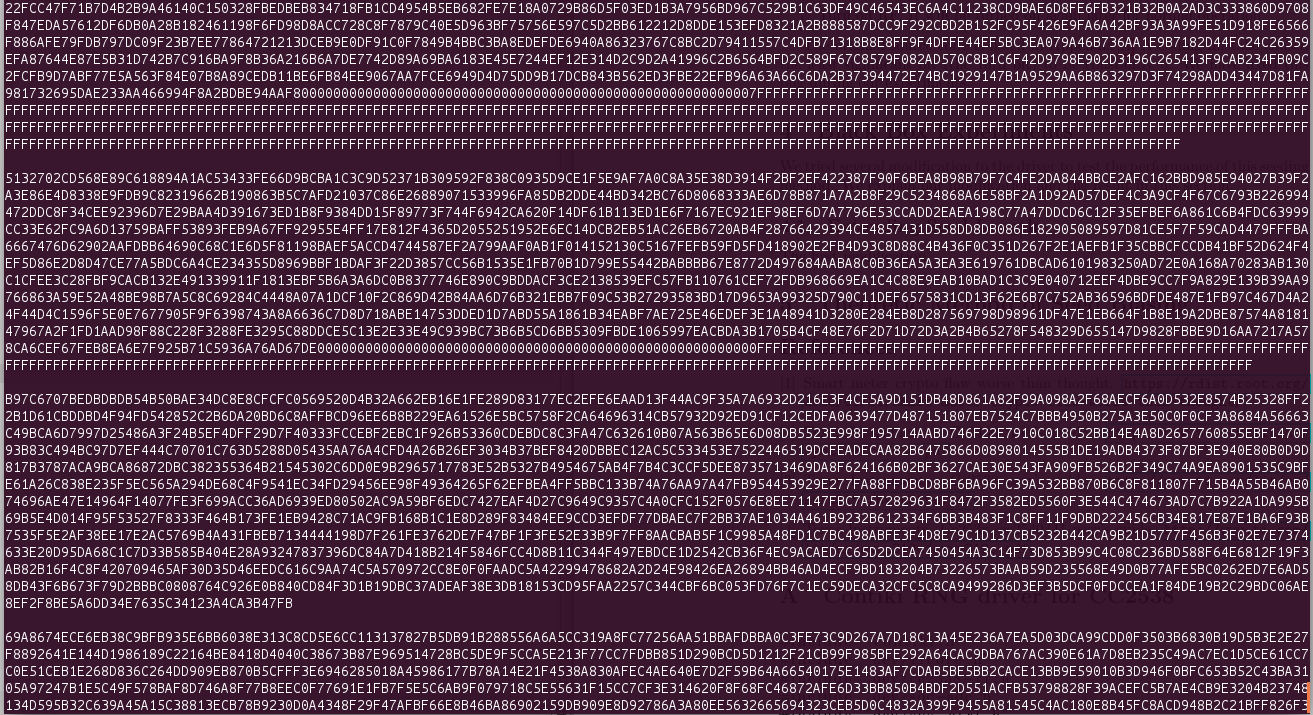
\includegraphics[width=\linewidth]{./figures/SeedExtend.png}
%\label{RFRND8096}
%\end{figure}
%
%\Cref{RFRND8096} shows part of the result. Occasionally RFRND falls into a broken state after some readings.  Under such state, it outputs purely 0 or 1 with  a potential flip after the beginning few bits as shown in \Cref{RFRND8096}. Extending the length of seed to 32768 bits, we realised the error happens in every seeding procedure.

\section{Generation of RFRND}

The description of the RFRND implementation on CC2540 (\Cref{CC2540 RND}) gave a hint that CC2538 may also have used the least significant bit of IF\_ADC, which is the analogue output of the mixer converted to digital. In this section we explain more details of how the bit is sampled.

\subsection{Mixer}

Mixer is a electric component used to convert a signal to lower or higher frequencies. A typical mixer is illustrated in \Cref{mixer}.

\begin{figure}
\center
\caption{Mixer Illustration}

\includegraphics[width=0.5\linewidth]{figures/mixer.png}
\label{mixer}
\end{figure}

The mixer takes two analogue input, RF and LO, and outputs IF which is the mixture of RF and LO. In our specific case,
\begin{itemize}
\item RF is the signal received by antenna amplified by LNA\footnote{Low Noise Amplifier}. For 802.15.4 communication, RF frequency $f_{R}$ is specified by 802.15.4 standard\cite{802154_Standard} as:
\begin{eqnarray}
f_{R} = 2405 + 5(k-11) [MHz] && k \in [11, 26]
\end{eqnarray}
where $k$ is the selectable channel number.

\item LO is a signal generated by the frequency synthesiser. The exact frequency of LO, denote as $f_{L}$, is adjusted according to required IF frequency.
\end{itemize}

An ideal mixer is implemented as the product of RF and LO. Denote the signals from RF and LO as $\cos(\omega_{R}t)$ and $\cos(\omega_{L}t)$ respectively, the IF output is:

\begin{equation} \label{IF}
\begin{split}
A_{R}\cos(\omega_{R}t)A_{L}\cos(\omega_{L}t) &= {\frac{A_{R}A_{L}}{2}}\cos((\omega_{R} + \omega_{L})t) + {\frac{A_{R}A_{L}}{2}}\cos((\omega_{R} - \omega_{L})t)
\end{split}
\end{equation} 

where $t$ is time and $\omega_i = 2{\pi}f_i$.

\Cref{IF} implies that there are two signals at IF, of one at frequency $(\omega_{R} + \omega_{L})$ and the other $(\omega_{R} - \omega_{L})$. In RF receiving path, the goal is to convert the high frequency signals into low frequency signals in order to be processed by local components; thus the signal at the higher frequency part in \Cref{IF} is then filtered by the band pass filters in both I and Q channels in \Cref{CC2430_RF}. 

Hence the input to IF\_ADC is:
\begin{equation}
x(t) = A'\cos((\omega_{R} - \omega_{L})t)
\end{equation}
where $A'$ is the amplitude adjusted by AGC. 

Denote $b$ as the random bit read from RFRND. One way to represent $b$ is:
\begin{equation} \label{RFRND}
b = \lfloor{x(t)} \mod 2V_0 \rfloor = \lfloor{A'\cos((\omega_{R} - \omega_{L})t) \mod 2V_0 }\rfloor
\end{equation}

where $V_0$ is the amount of measurement represented by the least significant bit of the ADC. The actual value of $b$ may be $\pm 1$ according to how ADC is implemented. Notice that \Cref{RFRND} does not take noise into account.

\subsection{Noise}

In real world deployment, the RF input is inevitably affected by several noise sources, include:

\begin{itemize}
\item Environmental radio noise.
\item Radio noise induced by the electronic system itself.
\item Approximation error within the system.
\end{itemize}

Denote $N(t)$ to be the noise in the input to IF\_ADC. Taking noise into account, \Cref{RFRND} should be rewritten as:

\begin{equation} \label{RFRND_noise}
\begin{split}
b &= \lfloor{(A'\cos((\omega_{R} - \omega_{L})t) + N(t) )\mod 2V_0 }\rfloor \\
&= \lfloor{(A'\cos((\omega_{R} - \omega_{L})t) \mod 2V_0 + N(t) \mod 2V_0 }\rfloor
\end{split}
\end{equation}

\Cref{RFRND_noise} suggests that any noise above $V_0$ may flip the bit $b$. According to CC2538 data sheet\cite{CC2538_Datasheet}, the RF receiver can be sensitive down to radio signals of $-97$dBm, whereas in our testing office environment, i.e. with multiple electronic devices and strong WiFi signal presented, the environmental noise easily exceeds this level. By nature noise is practically difficult to control, this poses a great difficulty when trying to manipulate the RFRND output.

\section{Bias Seeding}

As a matter of fact, a jamming signal is usually much stronger than the sensitivity of CC2538 ($-97$ dBm). In practice it is difficult to control such micro level voltage due to device limitation such as distortion of DAC.

On the other hand, the exact time of kernel accessing RFRND is unpredictable and IF\_ADC is buffered; implies that in order to bias RFRND, one would need to sustain a biased IF\_ADC output for a certain period. In this section, we discuss some potential methods to achieve this requirement.

\subsection{Noise Cancelling}

If the jamming signal can exactly cancel the noise including those generated by the device itself than we would expect RFRND to be biased, normally towards $0$. However I do not possess the technique to proceed this method.

Compensatory, one can put the device into a shielding box to eliminate environmental noise but it cannot shield the noise generated by the device itself.

\subsection{Ground RF}

Ideally by connecting RF to the signal earth we expect to reduce the input of IF\_ADC to $0$, resulting into a constant output to RFRND. But in practice, jumping over such integrated devices seems to be difficult.

\subsection{Saturate IF\_ADC}

When an input voltage equal to or higher than the maximum allowance is given, the many ADC design is expected to output a fixed maximum value $V_{max}$. The idea is to send a jamming signal that is strong enough to saturate the ADC and thus bias RFRND.

There are several concerns in this method.  The first and greatest concern is that saturating the RF input may permanently damage the device due to excessive voltage. Secondly, the actual input voltage is adjusted by AGC; therefore it is uncertain how the jamming signal strength will be preserved at the ADC input. Also if the required signal strength exceeded any allowed input of the components in the RF receive path, the result could be unpredictable.

One way to design the jamming signal is to simply set its frequency to exactly the frequency used for normal communication to pass the band pass filter. The strength of signal is controlled by the IF\_GAIN of the jamming device. Ideally RFRND is expected to have a predictable output whenever RF input is saturated, as depicted in \Cref{Saturate_ADC}.

\begin{figure}
\center
\caption{Connecting RF to USB\_GND}
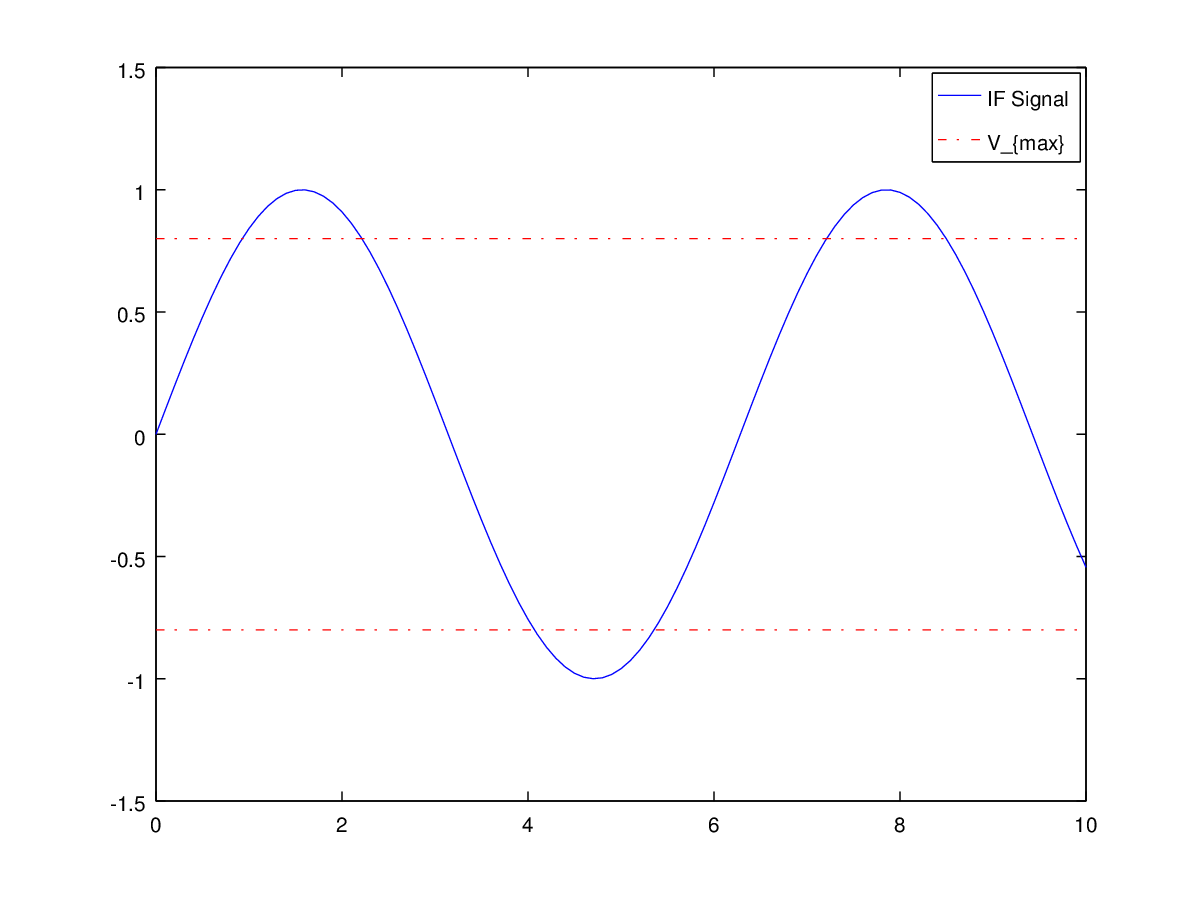
\includegraphics[width=\textwidth]{figures/saturate.png}
\label{UsbGnd}
\end{figure}

CC2538 data sheet specifies the maximum input level of RF receive to be $10$ dBm. I tried to directly connect the jamming device, a HackRF One, to the CC2538 powered device, an OpenMote Rev C, through a 5m SMA cable in order to increase the input to CC2538 RF. The maximum RSSI I have achieved is $-10$ dBm which is still $20$ dBm down the minimum required. The result suggests that perhaps an amplifier is needed for this method; but this again could be risky to both devices.

\subsubsection{Connecting RF to USB\_GND}

As an alternative attempt, we tried to connect the antenna of OpenMote to the GND pin on the base board as shown in \Cref{UsbGnd}. In our setup, USB cable is used as the power source of the device; thus we expect a constant input to RF of which equals to the difference between the chassis ground and signal ground. 

\begin{figure}
\center
\caption{Connecting OpenMote Antenna to GND Pin}
\includegraphics[width=\textwidth]{figures/usb_gnd.jpg}
\label{UsbGnd}
\end{figure}

We collected $1180901$ bits under this setup and ran them through the NIST test suite. Comparing to \Cref{NIST test}, these bits failed several some of the tests including:

\begin{itemize}
\item Frequency Test\cite{NistTestSuite}.
\item Cumulative Sums (Forward) Test\cite{NistTestSuite}.
\item Cumulative Sums (Reverse) Test\cite{NistTestSuite}.
\item Maurer's ``Universal Statistical'' Test\cite{NistTestSuite}. 
\end{itemize}

Specifically, the frequency of bit $0$ has slightly decreased to $P(0) = 49.5868\%$, suggesting this method could have biased the seeding towards $1$ by roughly $0.35\%$. The full report of this test is given in \Cref{GroundedReport}.